\documentclass{article}
\usepackage{graphicx} % Required for inserting images
\usepackage{authblk} % Required for author affiliations
\usepackage{indentfirst} % Indent first paragraph of sections
\usepackage{amssymb} % For mathematical symbols
\usepackage{amsthm} % For theorem environments
\usepackage{amsmath} % For advanced math typesetting
\usepackage[hidelinks]{hyperref}
\usepackage{enumitem}
\usepackage{pgfplots} % For plots
\pgfplotsset{compat=1.18} % Set compatibility level
\usepackage{tikz} % For drawing shapes
\newtheorem{theorem}{Theorem}
\newtheorem{corollary}{Corollary}[theorem]
\newtheorem{lemma}[theorem]{Lemma}
\newtheorem{definition}{Definition}
\newtheorem{problem}{Problem}
\newtheorem{solution}{Solution}
\newtheorem{example}{Example}
\newtheorem{remark}{Remark}
\begin{document}
%------- Title page   -----------
\title{PHYS 241: Signal Processing}
\author{William Homier}
\affil[1]{McGill University Physics, 3600 Rue University, Montréal, QC H3A 2T8, Canada}
\date{January \(6^{th}\), 2026}
\setcounter{Maxaffil}{0}
\renewcommand\Affilfont{\itshape\small}
\maketitle

%------- Abstract -----------
\noindent\rule{\textwidth}{0.4pt}
\thispagestyle{empty}
\begin{abstract}
\end{abstract}
\noindent\rule{\textwidth}{0.4pt}
\clearpage

%------- Table of Contents -----------
\thispagestyle{empty}
\hypersetup{
    citecolor=black,
    filecolor=black,
    linkcolor=black,
    urlcolor=black
}
\tableofcontents
\clearpage

%------- introduction -----------
\setcounter{page}{1}
\section{Introduction}
\section{Prerequisite knowledge}
\section{Basics \& Voltage, Current and Resistance}
\subsection{Signal Types}
\subsubsection{Digital Signal}
\begin{definition}
    A discretely sampled signal with a sequence of quantized values.
\end{definition}
\subsubsection{Analogue}
\begin{definition}
    A continuous signal (e.g., in time) representing (analogous to) some other quantity.
\end{definition}
\begin{example}
    Examples of analogue devices and computers are:
    \begin{itemize}
        \item thermometers
        \item sextants
        \item tide-predicting machine
    \end{itemize}
\end{example}
\subsection{Circuits}
\subsubsection{DC}
\begin{definition}
    Direct Current (DC) is a form of current where voltage and current are constant over time.
\end{definition}
\paragraph{DC Offset}
We often talk about adding a \textbf{DC offset} to an AC signal.  
This means adding a constant DC value to an AC signal.  
Doing this shifts the entire signal up or down relative to the \(0\,\text{V}\) level, without changing the shape of the AC signal.

\begin{example}
    Example of a source of DC current is a battery.
\end{example}
\subsubsection{AC}
\begin{definition}
    Alternating Current (AC) is a form of current that changes over time, often in a sinusoidal manner.
\end{definition}
\begin{example}
    Example of a source of AC current is a transformer. Other examples of AC current are wall outlets.
\end{example}

\subsection{Waves}
\subsubsection{Properties of waves}
To describe waves, considering a sinusoidal wave of the form \(A_psin(2\pi vt)\), we use the following terms
\begin{itemize}
    \item Peak amplitude (\(A_p\)): maximum value of the wave from its equilibrium position .
    \item Peak-to-peak amplitude: total height of the wave from its maximum to its minimum value (i.e., \(2A_p\)).
    \item Frequency (\(v\)): number of cycles per second (Hz).
    \item Time (\(t\)): time variable.
\end{itemize}
To be able to describe AC signals effectively, we take the root mean square (RMS) amplitude \(\frac{A_p}{\sqrt{2}}\) of values such as current and voltage.
\[I_{RMS} = \frac{I_p}{\sqrt{2}}\]
\[V_{RMS} = \frac{V_p}{\sqrt{2}}\]

\subsubsection{Waveforms}

A waveform is the shape of a signal when plotted as a function of time. Common waveforms include:
\begin{itemize}
    \item Sine wave
    \item Square wave
    \item Triangle wave
    \item Sawtooth wave
\end{itemize}

\paragraph{Direct current (DC).}
A direct current is constant in time, so its graph is a horizontal line.

Graph of a direct current \(I(t)\):
\begin{center}
\begin{tikzpicture}[scale=1.1]
    % Axes
    \draw[->] (-0.5,0) -- (6,0) node[right] {$t$};
    \draw[->] (0,-0.5) -- (0,5) node[above] {$I(t)$};

    % DC graph
    \draw (0,3) -- (6,3);
\end{tikzpicture}
\end{center}

\paragraph{Alternating current (AC).}
An alternating current varies periodically in time and typically oscillates about zero.

Graph of an alternating current \(I(t)\):
\begin{center}
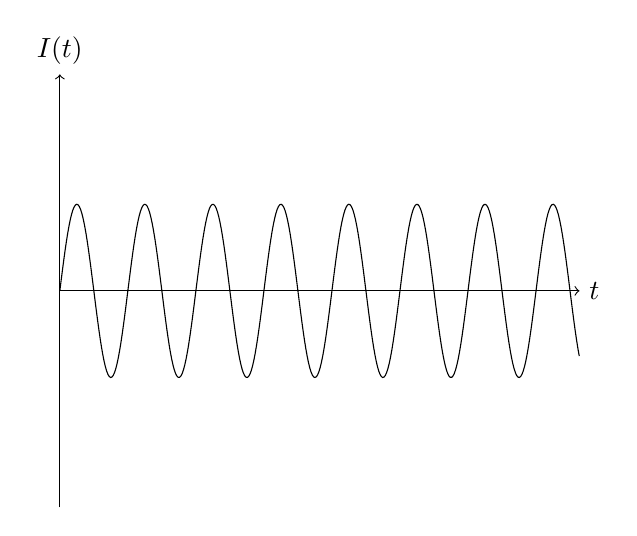
\begin{tikzpicture}[scale=1.1]
    % Axes
    \draw[->] (0,2.5) -- (6,2.5) node[right] {$t$};
    \draw[->] (0,0) -- (0,5) node[above] {$I(t)$};

    % AC graph
    \draw[domain=0:6, samples=400] plot (\x,{sin(8*\x r)+2.5});
\end{tikzpicture}
\end{center}

\paragraph{Pulsating current (DC + AC).}
A pulsating current is an alternating current superimposed on a non-zero DC level. This is just a matter of adding a constant DC level to an AC signal so that the signal is either shifted up or down with respect to the zero current level.

Graph of a pulsating current \(I(t)\):
\begin{center}
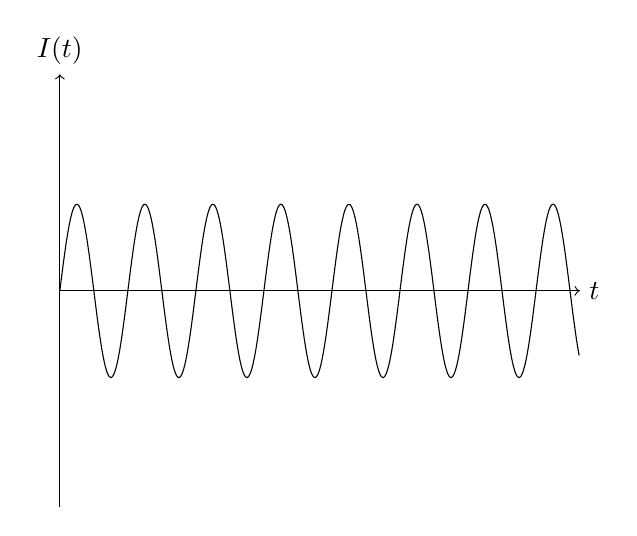
\begin{tikzpicture}[scale=1.1]
    % Axes
    \draw[->] (0,2.5) -- (6,2.5) node[right] {$t$};
    \draw[->] (0,0) -- (0,5) node[above] {$I(t)$};

    % AC + DC signal
    \draw[domain=0:6, samples=600] plot (\x,{sin(8*\x r)+2.5});

    % DC level
    \draw[dashed] (0,2.5) -- (6,2.5);
\end{tikzpicture}
\end{center}

\subsection{Linear Systems}
\begin{definition}
    Linear systems obey the principles of superposition and scaling.
\end{definition}
\begin{example}
    Consider two inputs $x_1(t)$ and $x_2(t)$ to a linear system producing outputs $y_1(t) = H[x_1(t)]$ and $y_2(t) = H[x_2(t)]$, where $H$ is some transformation function.

    A linear transformation must satisfy:
    \[y_{total} = \alpha y_1(t) + \beta y_1(t) = H[\alpha x_1(t) + \beta x_2(t)],\]
    where \(\alpha\) and \(\beta\) are constants.
\end{example}
\begin{example}[Superposition]
    \[H[x_1(t) + x_2(t)] = H[x_1(t)] + H[x_2(t)]\]
\end{example}
\begin{example}[Scaling]
    \[H[\alpha x(t)] = \alpha H[x(t)]\]
\end{example}
\subsection{Electric Charge}
\begin{definition}
    Charge is a fundamental physical property that comes in two types: positive (+) and negative (-) (which cancel). Positive and negative charge are usually present in matter in exactly equal proportion (so matter is typically electrically neutral). Charge is conserved—can neither be created nor destroyed and is quantized in units of electronic charge $e = 1.6 \times 10^{-19} \text{C}$.
\end{definition}
\subsection{Current flow}
\begin{definition}[Electric Current]
    Charge per unit time passing a given point in a circuit.
\end{definition}
\begin{definition}[Current Flow]
    The flow of electrons through a wire driven by an electric field potential energy difference. Defined as the rate of charge past a point in a circuit:
    \[I[ampere] = \frac{Q[coulomb]}{time[seconds]}\]
\end{definition}
\begin{definition}[Voltage]
    The electric potential energy divided by the charge. It is the energy per unit charge.
    \[V[volt] = \frac{\Delta E_{Electric}[joule]}{Q[coulomb]}\]
\end{definition}
\begin{definition}[Electron-volt]
    The energy gained or lost by an electron when it moves through an electric potential difference of one volt, which is a unit of energy equal to the work done on an electron in accelerating it through a potential difference of 1V, equal to $1.6 \times 10^{-19}$ Joule.
\end{definition}
\subsection{Ohm's Law}

\section{Circuit Theory Beyond Electronic}
\section{Capacitors \& Inductors}
\section{RC and LR Circuits with AC Driving}
\section{Impedance}
\section{RLC Circuits}
\subsection{Transient Response}
\subsection{Driven RLC Circuits}
\subsection{Power Input to RLC and Circuit Network}
\section{Circuit Networks}
\section{Fourier Series}
\section{Fourier Transforms}


\section{Appendix}

\section{Useful Links}

\end{document}